\documentclass[aspectratio=169,xcolor=dvipsnames]{beamer}
\usetheme{SimpleDarkBlue}

\usepackage{hyperref}
\usepackage{graphicx} % Allows including images
\usepackage{booktabs} % Allows the use of \toprule, \midrule and \bottomrule in tables


\title{Research Progress}
\subtitle{March 2025}

\author{Nithish Kumar V}

\institute
{
	Department of Computer Science and Engineering \\
	Indian Institute of Information Technology, Design and Manufacturing, Kancheepuram
}
\date{\today} 


\begin{document}
	
	\begin{frame}
		\titlepage
	\end{frame}
	
	\begin{frame}{Overview}
		\tableofcontents
	\end{frame}
	\section{Modelling Problems as Graphs}
	\begin{frame}{Modelling Problems as Graphs}
		\begin{itemize}
			\item Graphs for representing objects, complex interactions			
			\item Domains where the problems are modelled as graphs
			\begin{enumerate}
				\item Social Networks
				\item Chemical Compounds
				\item Knowledge Graphs
				\item Recommendation Systems
			\end{enumerate}
		\end{itemize}
	\end{frame}
	
	\section{Knowledge Graphs}
	\begin{frame}{Knowledge Graphs}
		\begin{itemize}
			\item A directed
			graph consisting of real-world facts, where the nodes function as the entities and the edges reflect the relations between the entities \cite{9996555}
		\end{itemize}
	\end{frame}
	%------------------------------------------------
	\section{Recommendation Systems}
	%------------------------------------------------
	
	\begin{frame}{Recommendation Systems}
		\begin{itemize}
			\item Recommendation is viewed as a system involving  \textbf{Users and Items}
			\item Basic models of Recommendation systems work with 2 kinds of data 
			\begin{enumerate}
				\item User Item Ratings
				\item Associated attributes of the user and items \cite{recsysbook}
			\end{enumerate}			 
		\end{itemize}
	\end{frame}
	\begin{frame}{Recommendation Systems}
		\begin{figure}
		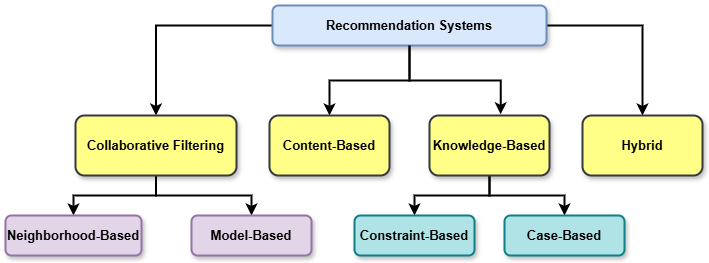
\includegraphics[width=0.8\linewidth]{recommendation systems taxanomy.png}
		\caption{Taxonomy of Recommendation Systems}
		\end{figure}
	\end{frame}
	
	
	%------------------------------------------------
	\section{Counterfactual Learning}
	%------------------------------------------------
	\begin{frame}{Counterfactual Learning}
		\begin{block}{Definition}
			Counterfactual Learning involves understanding how a model's prediction would change if specific input features were altered, essentially exploring "what-if" scenarios to understand a model's decision-making process. 
		\end{block}
		\begin{example}
			Consider a Loan Application system, where an application is rejected for a person with particular gender we can test the models outputs after altering the gender while keeping the values of all other attributes as same
		\end{example}
	\end{frame}
	
	\begin{frame}{Counterfactual Learning cont..}
		\begin{itemize}
		\item Counterfactuals are a fundamental and crucial concept within the framework of \textbf{Causal Inference}
		\item 2 main concepts
		\begin{enumerate}
			\item Counterfactual Fairness: prediction for an individual is 			fair if it remains the same in a counterfactual world where the individual belongs to a different demographic	group
			\item Counterfactual Explanation: provide actionable recommendations on what minimal 			changes to be made to alter the decision
		\end{enumerate}
		
		\end{itemize}
	\end{frame}
	\begin{frame}{Counterfactual Learning cont..}
		\begin{itemize}
			\item Main aim is to bring fairness and interpretability, extract additional information from the counterfactual world \cite{p1}
			\item Compared with traditional statistical models, causal 		models have better generalization ability in modeling real-world systems
			\item Counterfactuals also aid in augmenting data \cite{9950302}
		\end{itemize}
	\end{frame}
	\begin{frame}{Counterfactual Learning cont..}
		\begin{columns}[c] % The "c" option specifies centered vertical alignment while the "t" option is used for top vertical alignment
			
			\column{.45\textwidth} % Left column and width
			\begin{figure}
				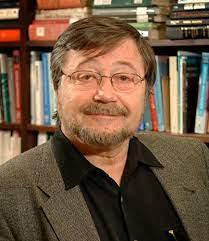
\includegraphics[width=0.8\linewidth]{judea pearl.jpg}
				\caption{Prof. Judea Pearl}
			\end{figure}
			
			\column{.45\textwidth} % Right column and width
			\begin{itemize}
				\item Recipient of the A.M. Turing Award
				\item  Credited for developing a theory of causal and counterfactual inference
			\end{itemize}
			
		\end{columns}
	\end{frame}
	\section{Counterfactual Learning on Graphs}
		
	
	\begin{frame}{Counterfactual Learning on Graphs}
		\begin{itemize}
			\item Recent works on graph counterfactual learning have shown great potential to overcome the aforementioned challenges 	on fairness, explanation, etc.
		\end{itemize}
	\end{frame}
	
	\begin{frame}{Benchmark Datasets}
			\begin{table}
				\begin{tabular}{l l}
					\toprule
					\textbf{Dataset} & \textbf{Domain} \\
					\midrule
					MovieLens         & Movie           \\
					LastFM         & Song           \\
					Book Crossing         & Book          \\
					FourSquares         & Location          \\
					Amazon Reviews         & Product          \\
					\bottomrule
				\end{tabular}
				\caption{Benchmark Datasets used in literature}
			\end{table}
	\end{frame}
	\begin{frame}{Tools, Frameworks}
		\begin{itemize}
			\item Pytorch Geometric - to train Graph Neural Networks (GNNs) for a wide range of applications
		\end{itemize}
	\end{frame}
	
	\begin{frame}{References}
		\footnotesize
		\bibliography{reference.bib}
		\bibliographystyle{apalike}
	\end{frame}
	
	\begin{frame}
		\Huge{\centerline{\textbf{The End}}}
	\end{frame}
	
	%----------------------------------------------------------------------------------------
	
\end{document}
